\PassOptionsToPackage{unicode=true}{hyperref} % options for packages loaded elsewhere
\PassOptionsToPackage{hyphens}{url}
%
\documentclass[
  ignorenonframetext,
]{beamer}
\usepackage{pgfpages}
\setbeamertemplate{caption}[numbered]
\setbeamertemplate{caption label separator}{: }
\setbeamercolor{caption name}{fg=normal text.fg}
\beamertemplatenavigationsymbolsempty
% Prevent slide breaks in the middle of a paragraph:
\widowpenalties 1 10000
\raggedbottom
\setbeamertemplate{part page}{
  \centering
  \begin{beamercolorbox}[sep=16pt,center]{part title}
    \usebeamerfont{part title}\insertpart\par
  \end{beamercolorbox}
}
\setbeamertemplate{section page}{
  \centering
  \begin{beamercolorbox}[sep=12pt,center]{part title}
    \usebeamerfont{section title}\insertsection\par
  \end{beamercolorbox}
}
\setbeamertemplate{subsection page}{
  \centering
  \begin{beamercolorbox}[sep=8pt,center]{part title}
    \usebeamerfont{subsection title}\insertsubsection\par
  \end{beamercolorbox}
}
\AtBeginPart{
  \frame{\partpage}
}
\AtBeginSection{
  \ifbibliography
  \else
    \frame{\sectionpage}
  \fi
}
\AtBeginSubsection{
  \frame{\subsectionpage}
}
\usepackage{lmodern}
\usepackage{amssymb,amsmath}
\usepackage{ifxetex,ifluatex}
\ifnum 0\ifxetex 1\fi\ifluatex 1\fi=0 % if pdftex
  \usepackage[T1]{fontenc}
  \usepackage[utf8]{inputenc}
  \usepackage{textcomp} % provides euro and other symbols
\else % if luatex or xelatex
  \usepackage{unicode-math}
  \defaultfontfeatures{Scale=MatchLowercase}
  \defaultfontfeatures[\rmfamily]{Ligatures=TeX,Scale=1}
\fi
% use upquote if available, for straight quotes in verbatim environments
\IfFileExists{upquote.sty}{\usepackage{upquote}}{}
\IfFileExists{microtype.sty}{% use microtype if available
  \usepackage[]{microtype}
  \UseMicrotypeSet[protrusion]{basicmath} % disable protrusion for tt fonts
}{}
\makeatletter
\@ifundefined{KOMAClassName}{% if non-KOMA class
  \IfFileExists{parskip.sty}{%
    \usepackage{parskip}
  }{% else
    \setlength{\parindent}{0pt}
    \setlength{\parskip}{6pt plus 2pt minus 1pt}}
}{% if KOMA class
  \KOMAoptions{parskip=half}}
\makeatother
\usepackage{xcolor}
\IfFileExists{xurl.sty}{\usepackage{xurl}}{} % add URL line breaks if available
\IfFileExists{bookmark.sty}{\usepackage{bookmark}}{\usepackage{hyperref}}
\hypersetup{
  pdftitle={SHINY},
  pdfauthor={Davi, Eduardo, Gabriela, Jadson, Tailine},
  pdfborder={0 0 0},
  breaklinks=true}
\urlstyle{same}  % don't use monospace font for urls
\newif\ifbibliography
\usepackage{color}
\usepackage{fancyvrb}
\newcommand{\VerbBar}{|}
\newcommand{\VERB}{\Verb[commandchars=\\\{\}]}
\DefineVerbatimEnvironment{Highlighting}{Verbatim}{commandchars=\\\{\}}
% Add ',fontsize=\small' for more characters per line
\usepackage{framed}
\definecolor{shadecolor}{RGB}{248,248,248}
\newenvironment{Shaded}{\begin{snugshade}}{\end{snugshade}}
\newcommand{\AlertTok}[1]{\textcolor[rgb]{0.94,0.16,0.16}{#1}}
\newcommand{\AnnotationTok}[1]{\textcolor[rgb]{0.56,0.35,0.01}{\textbf{\textit{#1}}}}
\newcommand{\AttributeTok}[1]{\textcolor[rgb]{0.77,0.63,0.00}{#1}}
\newcommand{\BaseNTok}[1]{\textcolor[rgb]{0.00,0.00,0.81}{#1}}
\newcommand{\BuiltInTok}[1]{#1}
\newcommand{\CharTok}[1]{\textcolor[rgb]{0.31,0.60,0.02}{#1}}
\newcommand{\CommentTok}[1]{\textcolor[rgb]{0.56,0.35,0.01}{\textit{#1}}}
\newcommand{\CommentVarTok}[1]{\textcolor[rgb]{0.56,0.35,0.01}{\textbf{\textit{#1}}}}
\newcommand{\ConstantTok}[1]{\textcolor[rgb]{0.00,0.00,0.00}{#1}}
\newcommand{\ControlFlowTok}[1]{\textcolor[rgb]{0.13,0.29,0.53}{\textbf{#1}}}
\newcommand{\DataTypeTok}[1]{\textcolor[rgb]{0.13,0.29,0.53}{#1}}
\newcommand{\DecValTok}[1]{\textcolor[rgb]{0.00,0.00,0.81}{#1}}
\newcommand{\DocumentationTok}[1]{\textcolor[rgb]{0.56,0.35,0.01}{\textbf{\textit{#1}}}}
\newcommand{\ErrorTok}[1]{\textcolor[rgb]{0.64,0.00,0.00}{\textbf{#1}}}
\newcommand{\ExtensionTok}[1]{#1}
\newcommand{\FloatTok}[1]{\textcolor[rgb]{0.00,0.00,0.81}{#1}}
\newcommand{\FunctionTok}[1]{\textcolor[rgb]{0.00,0.00,0.00}{#1}}
\newcommand{\ImportTok}[1]{#1}
\newcommand{\InformationTok}[1]{\textcolor[rgb]{0.56,0.35,0.01}{\textbf{\textit{#1}}}}
\newcommand{\KeywordTok}[1]{\textcolor[rgb]{0.13,0.29,0.53}{\textbf{#1}}}
\newcommand{\NormalTok}[1]{#1}
\newcommand{\OperatorTok}[1]{\textcolor[rgb]{0.81,0.36,0.00}{\textbf{#1}}}
\newcommand{\OtherTok}[1]{\textcolor[rgb]{0.56,0.35,0.01}{#1}}
\newcommand{\PreprocessorTok}[1]{\textcolor[rgb]{0.56,0.35,0.01}{\textit{#1}}}
\newcommand{\RegionMarkerTok}[1]{#1}
\newcommand{\SpecialCharTok}[1]{\textcolor[rgb]{0.00,0.00,0.00}{#1}}
\newcommand{\SpecialStringTok}[1]{\textcolor[rgb]{0.31,0.60,0.02}{#1}}
\newcommand{\StringTok}[1]{\textcolor[rgb]{0.31,0.60,0.02}{#1}}
\newcommand{\VariableTok}[1]{\textcolor[rgb]{0.00,0.00,0.00}{#1}}
\newcommand{\VerbatimStringTok}[1]{\textcolor[rgb]{0.31,0.60,0.02}{#1}}
\newcommand{\WarningTok}[1]{\textcolor[rgb]{0.56,0.35,0.01}{\textbf{\textit{#1}}}}
\setlength{\emergencystretch}{3em}  % prevent overfull lines
\providecommand{\tightlist}{%
  \setlength{\itemsep}{0pt}\setlength{\parskip}{0pt}}
\setcounter{secnumdepth}{-2}

% set default figure placement to htbp
\makeatletter
\def\fps@figure{htbp}
\makeatother

\usetheme[faculty=science, university=uu, logo=uu-logo]{fibeamer}
\usepackage{background}
\usepackage[absolute, overlay]{textpos}
\usepackage{ragged2e}  
\usepackage{booktabs}  
\usepackage{tabularx}
\usepackage{tikz}    
\usetikzlibrary{calc, shapes, backgrounds}
\usepackage{amsmath, amssymb}
\usepackage{url} 
\usepackage{listings}

\renewcommand{\baselinestretch}{1.5}
\newcommand{\RefTb}[1]{\textbf{Tabela~\ref{#1}}}
\newcommand{\RefFg}[1]{\textbf{Figura~\ref{#1}}}
\newcommand{\blackbox}{\rule{1.5ex}{1.5ex}}
\newcommand{\lp}{\left(}
\newcommand{\rp}{\right)}
\newcommand{\lch}{\left\{}
\newcommand{\rch}{\right\}}
\newcommand{\lc}{\left[}
\newcommand{\rc}{\right]}
\newcommand{\I}{1\!\!1}
\newcommand{\fimteo}{\hfill\rule[.5mm]{1ex}{1ex}}
\newcommand{\bff}[1]{\boldsymbol{#1}}
\newcommand{\rhob}{\bff{\rho}}
\newcommand{\kappab}{\bff{\kappa}}
\newcommand{\alphab}{\bff{\alpha}}
\newcommand{\betab}{\bff{\beta}}
\newcommand{\thetab}{\bff{\theta}}
\newcommand{\mub}{\bff{\mu}}
\newcommand{\gammab}{\bff{\gamma}}
\newcommand{\Gammab}{\bff{\Gamma}}
\newcommand{\varphib}{\bff{\varphi}}
\newcommand{\etab}{\bff{\eta}}
\newcommand{\zetab}{\bff{\zeta}}
\newcommand{\psib}{\bff{\psi}}
\newcommand{\Psib}{\bff{\Psi}}
\newcommand{\omegab}{\bff{\omega}}
\newcommand{\Sigmab}{\bff{\Sigma}}
\newcommand{\taub}{\bff{\tau}}
\newcommand{\pib}{\bff{\pi}}
\newcommand{\lambdab}{\bff{\lambda}}
\newcommand{\Lambdab}{\bff{\Lambda}}
\newcommand{\Deltab}{\bff{\Delta}}
\newcommand{\deltab}{\bff{\delta}}
\newcommand{\Imat}{\bff{\mathcal{I}}}
\newcommand{\phib}{\bff{\phi}}
\newcommand{\umb}{\bff{1}}
\newcommand{\zb}{\bff{0}}
\newcommand{\Ub}{\bff{U}}
\newcommand{\Cb}{\bff{C}}
\newcommand{\Sbl}{\bff{S}}
\newcommand{\sbl}{\bff{s}}
\newcommand{\Abl}{\bff{A}}
\newcommand{\Tb}{\bff{T}}
\newcommand{\Yb}{\bff{Y}}
\newcommand{\yb}{\bff{y}}
\newcommand{\Nb}{\bff{N}}
\newcommand{\nb}{\bff{n}}
\newcommand{\Ib}{\bff{I}}
\newcommand{\Hb}{\bff{H}}
\newcommand{\hb}{\bff{h}}
\newcommand{\Jb}{\bff{J}}
\newcommand{\Kb}{\bff{K}}
\newcommand{\Hbl}{\bff{H}}
\newcommand{\lb}{\bff{l}}
\newcommand{\Lb}{\bff{L}}
\newcommand{\xb}{\bff{x}}
\newcommand{\Xb}{\bff{X}}
\newcommand{\Wb}{\bff{W}}
\newcommand{\mb}{\bff{m}}
\newcommand{\Mb}{\bff{M}}
\newcommand{\Ab}{\bff{A}}
\newcommand{\ab}{\bff{a}}
\newcommand{\Bb}{\bff{B}}
\newcommand{\Pb}{\bff{P}}
\newcommand{\db}{\bff{d}}
\newcommand{\vb}{\bff{v}}
\newcommand{\tb}{\bff{t}}
\newcommand{\Vb}{\bff{V}}
\newcommand{\Db}{\bff{D}}
\newcommand{\Eb}{\bff{E}}
\newcommand{\Fb}{\bff{F}}
\newcommand{\fb}{\bff{f}}
\newcommand{\Rb}{\bff{R}}
\newcommand{\Zbl}{\bff{Z}}
\newcommand{\zbl}{\bff{z}}
\newcommand{\rb}{\bff{r}}
\newcommand{\bdot}{\bff{.}}
\newcommand{\varthetab}{\bff{\vartheta}}
\newcommand{\ini}{\noindent}
\newcommand{\inic}{\hspace{5.5mm}}
\newcommand{\mU}{\mathcal{U}}
\newcommand{\mS}{\mathcal{S}}
\newcommand{\EM}{\mathcal{E}}
\newcommand{\VM}{\mathcal{V}}
\newcommand{\Real}{\mathcal{R}}
\newcommand{\SA}{\mathcal{A}}
\newcommand{\MP}{\mathcal{P}}
\newcommand{\mpp}{{\it {p}}}
\newcommand{\ds}{\displaystyle}
\newcommand{\wthetab}{\widehat{\thetab}}
\newcommand{\wpib}{\widehat{\pib}}


\newcommand{\beq}{\begin{eqnarray}}
\newcommand{\eeq}{\end{eqnarray}}
\newcommand{\beqq}{\begin{eqnarray*}}
\newcommand{\eeqq}{\end{eqnarray*}}
\newcommand\mycom[2]{\genfrac{}{}{0pt}{}{#1}{#2}}

\title{SHINY}
\subtitle{INTERATIVIDADE COM R}
\author{Davi, Eduardo, Gabriela, Jadson, Tailine}
\date{}

\begin{document}
\frame{\titlepage}

\begin{frame}{SUMÁRIO}
\protect\hypertarget{sumario}{}

\begin{enumerate}
\item O que é o Shiny?
\item Estrutura básica
\begin{enumerate}
\item User Interface
\item Server
\end{enumerate}
\item Aplicações
\item Referências
\end{enumerate}

\end{frame}

\begin{frame}{}
\protect\hypertarget{section}{}

\begin{textblock*}{0cm}(0cm,-.0cm)

\includegraphics[width=\paperwidth, height=\paperheight]{imagens/logo}
\end{textblock*}

\end{frame}

\begin{frame}{INTERATIVIDADE}
\protect\hypertarget{interatividade}{}

\section{Instruções do Servidor (R)}
\begin{center}
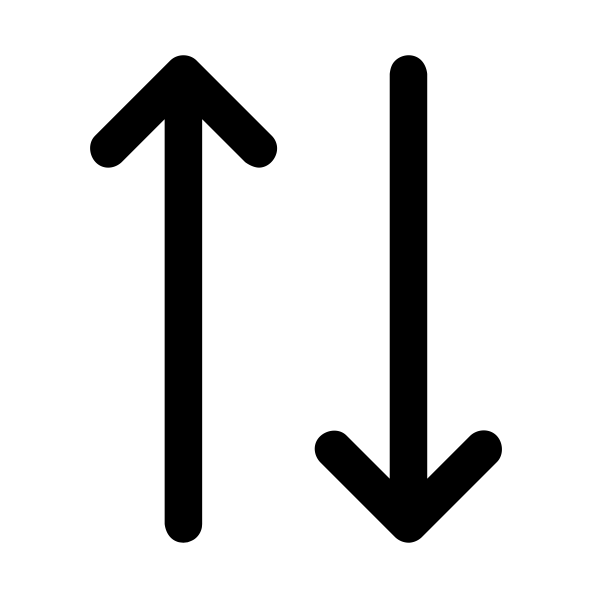
\includegraphics[width=13mm]{imagens/trade}
\end{center}
\section{User Interface (UI)}

\end{frame}

\begin{frame}{REATIVIDADE}
\protect\hypertarget{reatividade}{}

\begin{figure}
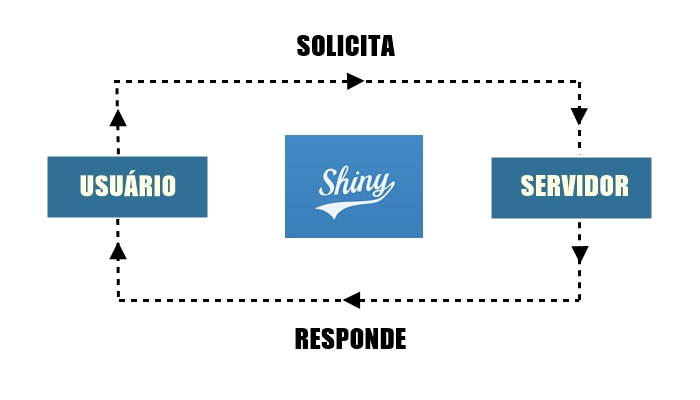
\includegraphics[width=110mm]{imagens/cxv}
\end{figure}

\end{frame}

\begin{frame}{RESUMINDO}
\protect\hypertarget{resumindo}{}

\begin{itemize}
\item Pacote do R
\item Cria de um servidor que envia páginas web, \textbf{recebe} informações do usuário e \textbf{processa} os dados.
\item Permite estruturar a interface do usuário \textbf{e} o processamento de dados.
\item Vantagens para o programador e para o usuário.
\end{itemize}

\end{frame}

\begin{frame}[fragile]{ESTRUTURA}
\protect\hypertarget{estrutura}{}

\begin{Shaded}
\begin{Highlighting}[]
\KeywordTok{library}\NormalTok{(shiny)}

\NormalTok{ui <-}\StringTok{ }\KeywordTok{fluidPage}\NormalTok{()}

\NormalTok{server <-}\StringTok{ }\ControlFlowTok{function}\NormalTok{(input, output) \{\}}

\KeywordTok{shinyApp}\NormalTok{(}\DataTypeTok{ui =}\NormalTok{ ui, }\DataTypeTok{server =}\NormalTok{ server)}
\end{Highlighting}
\end{Shaded}

\end{frame}

\begin{frame}{USER INTERFACE (UI)}
\protect\hypertarget{user-interface-ui}{}

\begin{table}
\begin{tabular}{l | l}
Função & Finalidade \\
\hline \hline
library(shiny) & \small Carregar o pacote Shiny. \\
ui <- fluidPage() & \small Criar uma interface com o usuário. \\
titlePanel() & \small Criar um painel contendo um título do aplicativo. \\
sidebarLayout() & \small Criar um layout com uma barra lateral e área principal. \\
sidebarPanel() & \small Criar um painel com barra lateral. \\
mainPanel() & \small Criar um painel principal contendo elementos de saída. \\
\end{tabular}
\end{table}

\end{frame}

\begin{frame}{WIDGETS}
\protect\hypertarget{widgets}{}

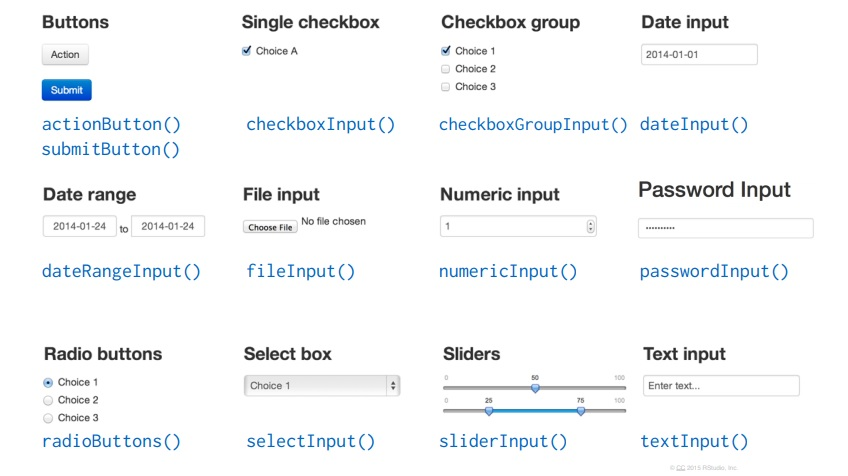
\includegraphics[width=4.4in]{imagens/inpfun}

\begin{center}
\tiny{Fonte: Shiny from RStudio}
\end{center}

\end{frame}

\begin{frame}[fragile]{CRIANDO FUNÇÕES DE ENTRADA}
\protect\hypertarget{criando-funcoes-de-entrada}{}

\only<2>{
\begin{textblock}{1}[0, .5](1.7, 8.5)
\begin{tikzpicture}
    \draw[fibeamer@red, ultra thick,rounded corners] (0,0) rectangle (6.8,2.1);
\end{tikzpicture}
\end{textblock}
}

\begin{Shaded}
\begin{Highlighting}[]
\KeywordTok{library}\NormalTok{(shiny)}
\NormalTok{ui <-}\StringTok{ }\KeywordTok{fluidPage}\NormalTok{(}
  \KeywordTok{sliderInput}\NormalTok{(}\DataTypeTok{inputId =} \StringTok{"num"}\NormalTok{,}
              \DataTypeTok{label =} \OtherTok{NULL}\NormalTok{,}
              \DataTypeTok{value =} \DecValTok{25}\NormalTok{, }\DataTypeTok{min =} \DecValTok{1}\NormalTok{, }\DataTypeTok{max =} \DecValTok{100}\NormalTok{) )}
\NormalTok{server <-}\StringTok{ }\ControlFlowTok{function}\NormalTok{(input, output) \{\}}
\KeywordTok{shinyApp}\NormalTok{(}\DataTypeTok{ui =}\NormalTok{ ui, }\DataTypeTok{server =}\NormalTok{ server)}
\end{Highlighting}
\end{Shaded}

\end{frame}

\begin{frame}{PRÓXIMO PASSO}
\protect\hypertarget{proximo-passo}{}

\begin{center}
Para que seja possível \alert{visualizar} o input, é necessário escolher como será o \alert{output.}
Para esse exemplo, queremos que o output gere um \alert{gráfico.}
Mas que \alert{função} precisamos usar agora?
\end{center}

\end{frame}

\begin{frame}{OUTPUTS}
\protect\hypertarget{outputs}{}

\begin{table}
\begin{tabular}{l | l}
Função & Finalidade \\
\hline \hline
dataTableOutput() &  Tabela Interativa \\
htmlOutput() & HTML puro \\ 
imageOutput() & Imagem \\
plotOutput() & Gráfico \\
tableOutput() & Tabela \\
textOutput() & Texto \\
uiOutput() & Elemento do Shiny UI \\
verbatimTextOutput() & Texto \\
\end{tabular}
\end{table}

\end{frame}

\begin{frame}[fragile]{DEFININDO O TIPO DE OUTPUT}
\protect\hypertarget{definindo-o-tipo-de-output}{}

\only<2>{
\begin{textblock}{1}[0, .5](1.7, 10.5)
\begin{tikzpicture}
    \draw[fibeamer@red, ultra thick,rounded corners] (0,0) rectangle (5,.7);
\end{tikzpicture}
\end{textblock}
}

\begin{Shaded}
\begin{Highlighting}[]
\KeywordTok{library}\NormalTok{(shiny)}
\NormalTok{ui <-}\StringTok{ }\KeywordTok{fluidPage}\NormalTok{(}
  \KeywordTok{sliderInput}\NormalTok{(}\DataTypeTok{inputId =} \StringTok{"num"}\NormalTok{,}
              \DataTypeTok{label =} \OtherTok{NULL}\NormalTok{,}
              \DataTypeTok{value =} \DecValTok{25}\NormalTok{, }\DataTypeTok{min =} \DecValTok{1}\NormalTok{, }\DataTypeTok{max =} \DecValTok{100}\NormalTok{), }
  \KeywordTok{plotOutput}\NormalTok{(}\StringTok{"hist"}\NormalTok{))}
\NormalTok{server <-}\StringTok{ }\ControlFlowTok{function}\NormalTok{(input, output) \{\}}
\KeywordTok{shinyApp}\NormalTok{(}\DataTypeTok{ui =}\NormalTok{ ui, }\DataTypeTok{server =}\NormalTok{ server)}
\end{Highlighting}
\end{Shaded}

\end{frame}

\begin{frame}{RESULTADO}
\protect\hypertarget{resultado}{}

\begin{center}
      Agora foi gerado um \alert{botão de slide} onde o usuário fará a escolha de um número entre 1 e 100.\\\bigskip
    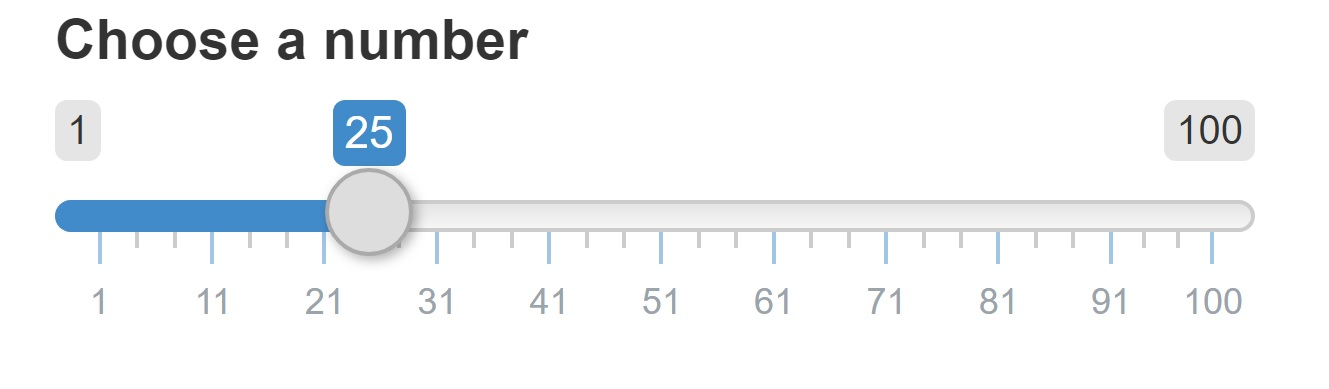
\includegraphics[width=75mm]{imagens/p1}
\end{center}

\end{frame}

\begin{frame}{PRÓXIMO PASSO}
\protect\hypertarget{proximo-passo-1}{}

\begin{center}
A próxima etapa é \alert{configurar} o output.
\end{center}
\begin{center} 
Dentro do UI, apenas demos alguns nomes.
\end{center}
\begin{center}
Agora precisamos definir o que realmente vai acontecer.
\end{center}

\end{frame}

\begin{frame}{SERVER}
\protect\hypertarget{server}{}

\begin{table}
\begin{tabular}{l | l}
Função & Finalidade \\
\hline \hline
library(shiny) & \small Carregar o pacote Shiny. \\
shinyServer() & \small Definir a lógica do servidor do aplicativo Shiny. \\ 
function(input,output){} & \small Funções render() \\
\end{tabular}
\end{table}

\end{frame}

\begin{frame}{RENDER ()}
\protect\hypertarget{render}{}

\begin{table}
\begin{tabular}{l | l}
Output (UI) & Render (Server) \\
\hline \hline
dataTableOutput() &  renderDataTable \\
imageOutput() & renderImage \\
plotOutput() & renderPlot \\
tableOutput() & renderTable \\
textOutput() & renderText \\
verbatimTextOutput() & renderPrint \\
uiOutput() & renderUI\\
htmlOutput() & renderUI \\ 
\end{tabular}
\end{table}

\end{frame}

\begin{frame}[fragile]{CONFIGURANDO O OUTPUT}
\protect\hypertarget{configurando-o-output}{}

\only<2>{
\begin{textblock}{1}[0, .5](1.7, 12.2)
\begin{tikzpicture}
    \draw[fibeamer@red, ultra thick,rounded corners] (0,0) rectangle (5.7,1.5);
\end{tikzpicture}
\end{textblock}
}

\begin{Shaded}
\begin{Highlighting}[]
\KeywordTok{library}\NormalTok{(shiny)}
\NormalTok{ui <-}\StringTok{ }\KeywordTok{fluidPage}\NormalTok{(}
  \KeywordTok{sliderInput}\NormalTok{(}\DataTypeTok{inputId =} \StringTok{"num"}\NormalTok{,}
              \DataTypeTok{label =} \OtherTok{NULL}\NormalTok{,}
              \DataTypeTok{value =} \DecValTok{25}\NormalTok{, }\DataTypeTok{min =} \DecValTok{1}\NormalTok{, }\DataTypeTok{max =} \DecValTok{100}\NormalTok{), }
  \KeywordTok{plotOutput}\NormalTok{(}\StringTok{"hist"}\NormalTok{))}
\NormalTok{server <-}\StringTok{ }\ControlFlowTok{function}\NormalTok{(input, output) \{}
\NormalTok{  output}\OperatorTok{$}\NormalTok{hist <-}\StringTok{ }\KeywordTok{renderPlot}\NormalTok{(\{}
    \KeywordTok{hist}\NormalTok{(}\KeywordTok{rnorm}\NormalTok{(input}\OperatorTok{$}\NormalTok{num))\})\}}
\KeywordTok{shinyApp}\NormalTok{(}\DataTypeTok{ui =}\NormalTok{ ui, }\DataTypeTok{server =}\NormalTok{ server)}
\end{Highlighting}
\end{Shaded}

\end{frame}

\begin{frame}{RESULTADO}
\protect\hypertarget{resultado-1}{}

\begin{columns}
  \centering
    \column{0.5\textwidth}
      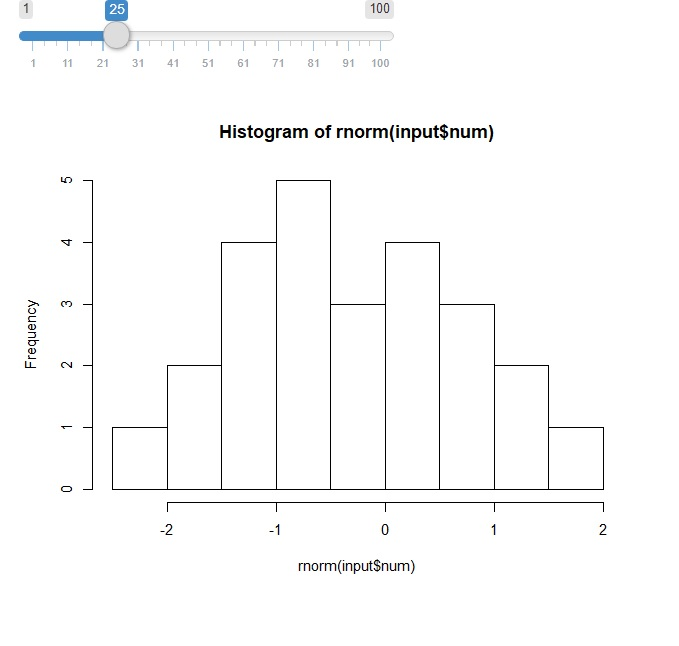
\includegraphics[width=50mm]{imagens/p2}
    \column{0.5\textwidth}
      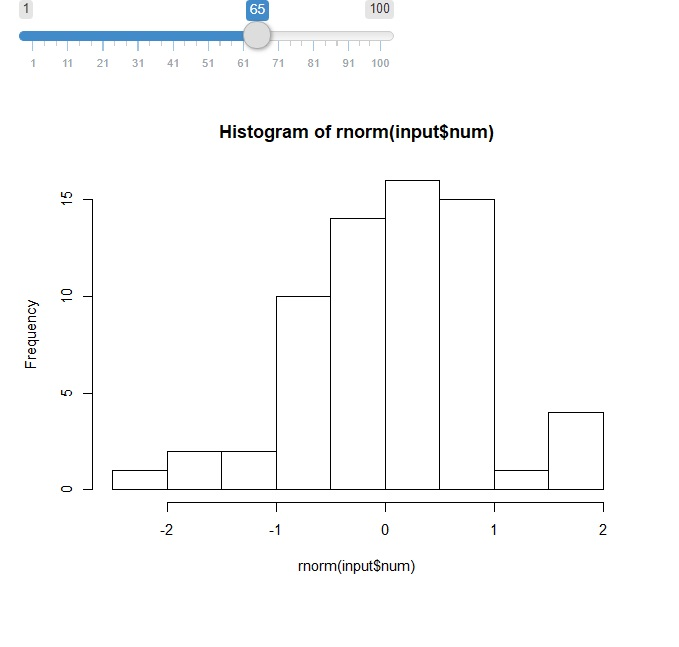
\includegraphics[width=50mm]{imagens/p3}
\end{columns}

\end{frame}

\hypertarget{aplicacoes}{%
\section{APLICAÇÕES}\label{aplicacoes}}

\begin{frame}{REFERÊNCIAS}
\protect\hypertarget{referencias}{}

\begin{enumerate}
\tightlist
\item
  RSTUDIO INC. \textbf{Shiny from RStudio}. Disponível em:
  \url{https://shiny.rstudio.com/tutorial/}. Acesso em: setembro de
  2019.
\item
  PUC MINAS. \textbf{Desenvolvimento de Aplicativos Web Com R e Shiny:}
  inovações no ensino de Estatística. Belo Horizonte,v. 6, n.~2,
  p.~55-71, maio 2018
\item
  \textbf{Curso-R}. Disponível em:
  \url{http://material.curso-r.com/shiny/}. Acesso em: setembro de 2019.
\end{enumerate}

\end{frame}

\end{document}
